\chapter[Lecture 19]{}\label{lec19}

From neutron scattering experiment, determine the energy of the loss feature as a function of \fbox{$\Delta k=k-k'$} that gives the dispersion of phonons.

Choose $G$ such that $\overrightarrow{k}$ lies in first Brillouin Zone. Plot $E$ vs. $K$.
\begin{figure}[H]
\centering
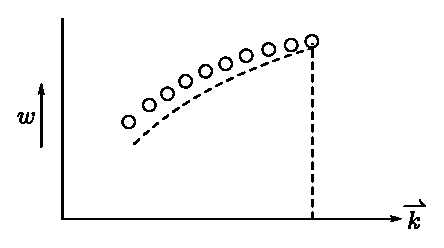
\includegraphics{images/lecture19/fig1a.eps}
\end{figure}

\section*{Specific Heat/Heat Capacity}

Heat Capacity : The amounting heat required to increase the temperature a system of unit mass by unity.

With change in temperature, other physical parameters also change, such as pressure, volume.

So, there are two quantities defined, one at constant volume and the other at constant pressure.
$$
C_{r}=\left(\dfrac{\partial U}{\partial T}\right)_{V}\quad U=\text{ internal energy.}
$$
This comes from,
$$
\delta Q=\delta U + p\delta V\quad \left(\dfrac{\partial Q}{\partial T}\right)_{V}=\left(\dfrac{\partial V}{\partial T}\right)_{V}
$$
$C_{P}=\left(\dfrac{\partial H}{\partial T}\right)_{P}$ \ $H$ is enthalpy of the system (total heat content)
\begin{align*}
&= U+PV\\
\delta H &= \delta V+P\delta V+V\delta P=\delta Q+V\delta P\\
\Rightarrow \left(\dfrac{\partial H}{\partial T}\right)_{P} &= \left(\dfrac{\partial Q}{\partial T}\right)_{P}=C_{P}
\end{align*}
$\to$ Although measurements are often done at constant pressure, heat capacity at constant volume is more fundamental and involves internal energy. So we focus mostly on $C_{V}$. $C_{P}$ can be calculated from $C_{V}$
$$
C_{P}-C_{V}=T\left(\dfrac{\partial P}{\partial T}\right)_{V,n}\left(\dfrac{\partial V}{\partial t}\right)_{P.n}
$$
$$
\fbox{$w_{k,p}=\sqrt{\dfrac{2C_{P}}{M}}\sqrt{1-\cos ka_{P}}$}
$$
Contribution of phonons to heat capacity is called lattice heat capacity, $C_{lot}$.

Total internal energy due to phonons can be written as
$$
U=\sum\limits_{k,p}U_{k,p}=\sum\limits_{k,p}\langle n_{k,p}\rangle \hbar w_{kp}
$$
$\langle n_{kp}\rangle$ is the thermal equilibrium occupancy of phonons of wave vector $k$ and polarization $p$.

Using Planck's distance function one can write
$$
\fbox{$\langle n\rangle = \dfrac{1}{e^{\hbar w/k_{B^{T}}}-1}$}
$$

\begin{proof}
Consider a set of identical harmonic oscillators in thermal equilibrium.

The ratio of the number of oscillator in their $(n+1)$th quantum state of excitation to the number in $n^{\text{th}}$ quantum state is
$$
N_{n+1}/N_{n}=e^{-\hbar w/k_{B^{T}}}\quad \dfrac{1}{k_{B^{T}}}=\beta
$$
$\therefore \ $ fraction of total no. of oscillator at $n^{\text{th}}$ state is
$$
\dfrac{N_{n}}{\sum\limits^{\infty}_{n=0}N_{n}}=\dfrac{e^{-n\hbar w\beta}}{\sum\limits^{\infty}_{n=0}e^{-n\hbar w\beta}}\quad\text{and}\quad 
\fbox{$\langle n\rangle = \dfrac{\sum ne^{-n\hbar w\beta}}{\sum e^{-n\hbar w\beta}}$}
$$
\begin{align*}
\sum x^{n}&=\dfrac{1}{1-x};\quad \sum nx^{n}=x\dfrac{d}{dx}\sum x^{n}\\
&= \dfrac{x}{(1-x)^{2}}
\end{align*}
\begin{gather*}
a_{1}\langle n\rangle =\dfrac{x}{1-x};\quad x=e^{-\beta \hbar w}\\
a, \ \fbox{$\langle n\rangle = \dfrac{1}{e^{\hbar w\beta}-1}$}\\
\therefore \ U = \sum\limits_{kp}\dfrac{\hbar w_{kp}}{e^{\hbar w_{kp}\beta}-1}
\end{gather*}
One can change sum over $k$ to an integral.

If $D_{p}(w)dw$ is the no. of modes for polarization, $p$ and frequency range $w$ to $w+dw$

Then
$$
\fbox{$U=\sum\limits_{p}\int dw \ D_{p}(w)\dfrac{\hbar w}{e^{\hbar w\beta}-1}$}
$$
Lattice heat capacity will be $\dfrac{\partial U}{\partial T}$.
$$
a \ e_{V}=C_{lat}=k_{B}\sum\limits_{p}\int dw \ D_{p}(w)\dfrac{(\beta \hbar w)^{2}e^{\beta\hbar w}}{\left(e^{\beta \hbar w}-1\right)^{2}}
$$
$D_{p}(w)$ is the number of modes per unit frequency range or density of modes or density of states.
\end{proof}

\section*{Density of states}
\begin{figure}[H]
\centering
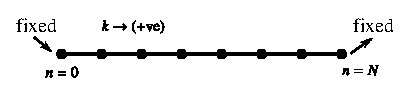
\includegraphics[scale=1.2]{images/lecture19/fig2a.eps}
\end{figure}

Take a one-dimensional chain of length $L$ and $(N+1)$ atoms. If the atoms at the end are kept fixed. There will be nodes for $n=0$ and $n=N$.
$$
u_{n}=u_{0}e^{-iw_{kp}t}\sin (nka)\quad a= \text{lattice constant.}
$$
Largest value of $k=\dfrac{2\pi}{a}$ and smallest value apart from `$0$' is $\dfrac{\pi}{L}$
$$
k\to \dfrac{\pi}{L}, \dfrac{2\pi}{L}, \dfrac{3\pi}{L},\ldots \dfrac{(N-1)\pi}{L}
$$
\begin{itemize}
\item For $k=\dfrac{N\pi}{L}=\dfrac{\pi}{a}$, $u_{s}L\sin n\pi=0$, so no motion for any atom.

\item Similarly for $k=0$, no motion.

$\therefore$ Total $(N-1)$ allowed modes are possible

= No. of atoms can move. (one mode per mobile atom)

\item Each allowed $k$ corresponds to a standing wave.

\item There is one mode for each interval of $\Delta k=\dfrac{\pi}{L}$

$\therefore$ No. of modes per unit $k$-range is $\dfrac{L}{\pi}$ for $k\leq \dfrac{\pi}{a}$

$0$ for $k>\dfrac{\pi}{a}$

\item There are three polarization for each of [one longitudinal two transverse] for one dimensional system.

\item In 3 dimensions, the same treatment for polarization works for certain $k$-direction.

\item If the medium is unbound, we can always find a distance `$L$' where both ends have same phase 

$\to \ $ use periodic boundary conditions
$$
\fbox{$u(na)=u(na+L)$}
$$
For the wave $u_{n}=u_{0}\exp [i(nka-w_{k}t)]$ the allowed $k$-values are $k=0$, $\pm\dfrac{2\pi}{L}$, $\pm \dfrac{4\pi}{L}$, $\pm \dfrac{6\pi}{L},\ldots,\dfrac{N\pi}{L}$

Here, $\Delta k=\dfrac{2\pi}{L}$ corresponds to each mode, and there are {\em two} values `$+$', `$-$'. Possible for each $k$.

No. of modes per unit range
\begin{align*}
\therefore\quad fk &= \dfrac{L}{2\pi}\quad\text{for}\quad -\dfrac{\pi}{a}\leq k\leq \dfrac{\pi}{a}\\
&= \text{~ otherwise.}
\end{align*}
No. of modes are same, one per mobile atom.

$D(w)=$ No. of modes per unit frequency range for a given polarization.
$$
\therefore\quad \fbox{$D(w)dw=\dfrac{L}{\pi}\dfrac{dk}{dw}\cdot dw=\dfrac{L}{\pi}\cdot \dfrac{dw}{(dw/dk)}$}\quad \dfrac{dw}{dk}=\text{ group velocity.}
$$
$\dfrac{dw}{dk}=v_{g}=$ group velocity; for $v_{g}=0$, There is singularity in $D(w)\to$ Van Hove Singularity.
\end{itemize}

\section*{Three dimension}
$$
\exp [i(k_{x}n+k_{y}y+k_{z}z)]=\exp [i\{k_{x}(x+L)+k_{y}(y+L)+k_{z}(z+L)\}]
$$
whence,
$$
k_{x},k_{y},k_{z}=0, \pm \dfrac{2\pi}{L}, \pm \dfrac{4\pi}{L}\ldots \dfrac{N\pi}{L}
$$
$\therefore$ One allowed $k$ per volume $\left(\dfrac{2\pi}{L}\right)^{3}$ in $k$-space.

$\therefore$ No. of allowed $k$ per unit volume = $\left(\dfrac{L}{2\pi}\right)^{3}=\dfrac{V}{8\pi^{3}}$ for each polarization and for each branch.

$\therefore$ Total No. of modes within $k$ a sphere of radius $k$ (modes with wave vector less than $k$)
\begin{gather*}
N=\left(\dfrac{L}{2\pi}\right)^{3}\cdot \dfrac{4\pi k^{3}}{3}\\
\therefore\quad \fbox{$D(w)=\dfrac{dN}{dw}=\dfrac{Vk^{2}}{2\pi^{2}}\cdot \dfrac{dk}{dw}$}
\end{gather*}

\section*{Specific Heat of a Classical Crystal}
$$
U=\dfrac{\int d\Gamma e^{-\beta H}\cdot H}{\int d\Gamma e^{-\beta}}\quad \beta=\dfrac{1}{k_{B}T}
$$
$\therefore$ \ Thermal energy density $=\dfrac{U}{V}=u=\dfrac{1}{V}\dfrac{\int d\Gamma e^{-\beta H}\cdot H}{\int d\Gamma e^{-\beta H}}$
\begin{gather*}
\text{or}\quad \fbox{$u=-\dfrac{1}{V}\dfrac{\partial}{\partial\beta} l_{a}\int d\Gamma e^{-\beta H}$}\\
H= \sum \dfrac{p(R)^{2}}{2M}+U^{eq}+U^{\text{Harm}}
\end{gather*}
\begin{align*}
d\Gamma &= \prod\limits_{R}du(R)dp(R)\\
&= \prod\limits_{R\mu}du_{\mu}(R)dp_{\mu}(R)
\end{align*}
If we substitute
\begin{align*}
u(R) &= \dfrac{1}{\sqrt{\beta}}u'(R)\\
p(R) &= \dfrac{1}{\sqrt{\beta}}p'(R)
\end{align*}
Then
\begin{align*}
\int d\Gamma e^{-\beta H} &= \int d\Gamma \exp \left[-\beta\left(\sum \dfrac{P(R)^{2}}{2M}+U^{eg}+U^{\text{Harm.}}\right)\right]\\
&= e^{-\beta U^{eg}}\cdot \beta^{-3N}\left\{\int\prod\limits_{R}du'(R)dp'(R)\right.\\
&\quad \left.\times \exp \left[-\sum \dfrac{1}{2M}p'(R)^{2}-\dfrac{1}{2}\sum u'_{\mu}(R)D_{\mu\nu}(R-R')u'_{\nu}(R)\right]\right\}
\end{align*}
$$
\therefore\quad u=-\dfrac{1}{V}\dfrac{\partial}{\partial\beta}l_{n}\left(e^{-\beta U^{eg}}\cdot \beta^{-3N}\times \text{Const}\right)=\dfrac{U^{eg}}{V}+\dfrac{3N}{V}k_{B}T
$$
\begin{align*}
a, u &= u^{eq}+3nk_{B}T\quad n>\dfrac{N}{V}\\
&= u^{eg}\quad\text{at}\quad T=0\text{~ static lattice theory}\\
\therefore \ C_{\nu} &= \dfrac{\partial u}{\partial T}=3nk_{B}
\end{align*}
$\therefore$ \ Specific heat due to just lattice vibrations is $3k_{B}$ per ion.

This is Dulong Petit law.

For monatomic solid $C_{V}=5.96 \text{ cal/mole.}k$

\section*{Experiment}
\begin{figure}[H]
\centering
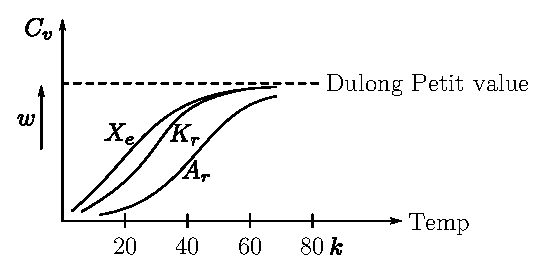
\includegraphics[scale=1.2]{images/lecture19/fig1.eps}
\end{figure}
\begin{itemize}
\item[(i)] $C_{v}$ decreases at low temperature, goes towards zero as $T\to 0$.

\item[(ii)] Even at high temperature, the difference is quite large.
\end{itemize}
So one needs to adopt quantum theory $\to$

(1910) study planck's radiation law, where phonon dispersion is \fbox{$w=vk$}.

\noindent
{\bf Debye model:} The velocity of sound is constant for each (1912) polarization type as it is for classical elastic continuum. 
\begin{align*}
\therefore \ w&= vk\quad v= \text{ velocity of sound.}\\
\therefore\quad D(w) &= \dfrac{Vk^{2}}{2\pi^{2}}\cdot \dfrac{dk}{dw}=\dfrac{Vw^{2}}{2\pi^{2}\nu^{3}}
\end{align*}
For monotomic solid dispersion of $w$ vs. $k$ is $w=\sqrt{\dfrac{4C}{M}}\left|\sin \dfrac{ka}{z}\right|$ for small $k$, $w$ and $k$.

If there are $N$ primitive calls in the specimen, total no. of acoustic phonon mode $=N$, one can determine {\em cut off frequency} $w_{D}$ as.
$$
\fbox{$w^{3}_{D}=\dfrac{6\pi^{2}\nu^{3}N}{V}$} \leftarrow N=\left(\dfrac{L}{2\pi}\right)^{3}\cdot \dfrac{4}{3}\pi k^{3}
$$
Cut off wave vector, $k_{D}=\dfrac{w_{D}}{\nu}=\left(\dfrac{6\pi^{2}N}{V}\right)^{\frac{1}{3}}$

In Debye model, modes larger than $k_{D}$ is not allowed.

Now
\begin{align*}
U &= \int dw \ D(w)\langle n(w)\rangle \hbar w\\
&= \int\limits^{w_{D}}_{0}dw\cdot \dfrac{Vw^{2}}{2\pi^{2}\nu^{3}}\cdot \dfrac{\hbar w}{e^{\beta\hbar w}-1}\text{~ for each polarization.}
\end{align*}
if $\nu$ is independent of polarization (assumption), for all the 3 polarizations, multiply by 3.
\begin{align*}
\therefore\quad U=\dfrac{3V\hbar}{2\pi^{2}\nu^{3}}\int\limits^{w_{D}}_{0}dw\cdot \dfrac{w^{3}}{e^{\beta \hbar w}-1} &= \dfrac{3Vk^{4}_{B}T^{4}}{2\pi^{2}\nu^{3}\hbar^{3}}\int\limits_{0}^{x_{D}}\dfrac{x^{3}}{e^{x}-1}\\
x = \beta\hbar w &= \dfrac{\hbar w}{k_{B}T}\\
x_{D}=\dfrac{\hbar w_{D}}{k_{B}T}=\dfrac{\theta}{T} \theta &= \text{ Debye temperature.}
\end{align*}
